\documentclass{article}
\usepackage[utf8]{inputenc}
\usepackage{listings}
\usepackage{graphicx}
\graphicspath{{images/}{../images/}}


\title{Concurrency \& Multithreading Summary}
\author{Jacob Burley}
\date{Block 1 2018}

\begin{document}

\maketitle

\tableofcontents
%
% Lecture 1
%
\section{Introduction}
Moore's law holds (more or less). The number of transistors on a chip doubles every two years. \textbf{But}:
\begin{itemize}
    \item As chip geometries shrink and clock frequencies rise, leakage current increases, leading to greater heat and power consumption
    \item memory acccess times haven't kept up with increasing clockspeeds, leading to a \textit{memory wall}
\end{itemize}
Multiprocessors combat this problem by combining multiple CPUs in a single system
\\Moore's law continues to be seen in parallelism, which also doubles every two years
\\Multicore processing is a challenge: at a \textbf{small scale}, processors within one chip must coordinate access to shared memory. At a \textbf{large scale}, processors in a supercomputer must coordinate handling and routing of data
\subsection{Symmetric Multiprocessing Architecture (SMP)}
Multiple processors with their own caches share access to a single memory, sharing the memory bus.
\\Example: Single socket multi-core CPU accesses a single bank of memory

\subsection{Non-Uniform Memory Access Architecture}
Multiple processors with their own caches \textbf{and} their own memory share their memory with eachother via inter-processor connections. Non-local memory access is \textbf{faster} if the memory you are requesting access to is physically closer to the requesting CPU.
\\Example: Multi-socket CPU accesses a bank of memory "belonging" to another CPU.
\subsection{Threads}
Threads are fully \textbf{asynchronous} - they do not exist (run) at the same time.
\begin{itemize}
    \item threads may be \textbf{delayed} or even \textbf{halted} without being warned by the system
    \item delays are unpredictable in both frequency and length
    \item there are 4 key kinds of delays:
    \begin{itemize}
        \item cache miss (short): thread expected something to be cached that wasn't, that item now needs to be fetched from main memory
        \item page fault (long): thread attempted to read from a page of memory that isn't currently addressable via virtual memory addresses. This page may now need to be loaded
        \item scheduling quantum used up (really long): Each thread gets an alloted time on the CPU per cycle. This delay means that a thread has used its time up. It must now wait until its next cycle to continue. Depending on the hardware capabilities and number of running threads, this might take some time.
        \item crashed (indefinite): The thread has crashed for some reason. If there is no way to recover the thread, this delay is indefinite.
    \end{itemize}
\end{itemize}
With \textbf{sequential computation}, a single thread processes instructions and modifies memory by itself.
\\With \textbf{concurrent computation}, multiple threads process instructions, and modify memory

\subsection{Safety and Liveness properties}
\textbf{Safety}: Something "bad" will never happen. I.e., mutual exclusion has a safety property as no two threads will ever have concurrent write access to the same variable.
\\\textbf{Liveness}: Something "good" will eventually happen, i.e. deadlock-free (if a pet wants to enter the garden, one of them eventually succeeds) or starvation-free (if a pet wants to enter the garden, it eventually succeeds)

\subsection{Progress Properties}
\textbf{Blocking}:
\begin{itemize}
    \item \textbf{Deadlock-free}: \textit{Some} thread trying to get the lock eventually succeeds
    \item \textbf{Starvation-free}: \textit{Every} thread trying to get the lock eventually succeeds.
\end{itemize}
\textbf{Non-blocking}:
\begin{itemize}
    \item \textbf{Lock-free}: \textit{Some} thread calling the method eventually returns.
    \item \textbf{Wait-free}: \textit{Every} thread calling the method eventually returns.
\end{itemize}
Lock/wait-free disallow the use of blocking methods such as locks, meaning they guarantee the system can cope with crash-failures.
\\Pick progress properties based on needs and what is possible.
\subsection{Alice and Bob, producer-consumer}
\begin{itemize}
    \item Bob must put food in garden when pets aren't there
    \item Alice only releases pets when there is food
    \item Bob only feeds when food runs out
\end{itemize}
\subsubsection{Can Protocol}
A can on Alice's window-sill, the string leads to Bob's house
\textbf{Alice's Protocol}:
\begin{itemize}
    \item wait until can is down
    \item release pets
    \item every time pets return, check whether there is food left
    \item if not: reset can, and keep pets inside until the can is down again
\end{itemize}
\textbf{Bob's Protocol}:
\begin{itemize}
    \item wait until the can (on Alice's window ledge) is up
    \item put food in the garden
    \item go inside, pull the string to knock down the can
\end{itemize}

\subsubsection{Can protocol correctness}
\textbf{Mutual Exclusion}: Bob and the pets are never in the yard together
\\\textbf{Starvation Free}: If Bob is always willing to feed, and Alice is always alert, pets are always full and eat infinitely often.
\\\textbf{Producer-consumer}: Pets only enter yard when there is food. Bob only enters yard when there \textit{isn't} food.

\subsection{Amdahl's Law}
Given a job that is executed on $n$ processors:
\\Let $p \in [0,1]$ be the fraction of the job that can be parallelized (over any $n$ of processors).
\\Let sequential execution of the job take 1 time unit.
\\Parallel execution of the job takes (at least) $(1-p)+\frac{p}{n}$ time units.
\\So, the speedup $S$ is 
$$\frac{1}{(1-p)+\frac{p}{n}}$$
\textbf{Example}:
$n=10$
\\$p=0.6$ gives speedup of $\frac{1}{0.4 + \frac{0.6}{10}}=2.2$
\\$p=0.9$ gives speedup of $\frac{1}{0.1 + \frac{0.9}{10}}=5.3$
\\$p=0.99$ gives speedup of $\frac{1}{0.01 + \frac{0.99}{10}}=9.2$
\\It can be seen that it is important to minimize sequential parts of a program in order to make efficient use of multiprocessors.






%
% Lecture 2
% Alice and Bob examples of mutexes from Lecture 1
%
\section{Mutual Exclusion}
\subsection{Events}
Threads exhibit sequences of events $a_0, a_1, a_2,...$ (e.g read/write to variable /invoke or return from a method).
\bigbreak Events are instantaneous, and \textit{never simultaneous}. (We can break ties between "simultaneous" events)
\bigbreak Consider the events of an execution by a multicore system:
$a\rightarrow b$ denotes that $a$ happens before $b$. This is \textit{total order}\footnote{Total Order: Any two elements of a set are comparable.}.
\bigbreak Let $a$ and $b$ be events by the \textit{same thread}, with $a \rightarrow b$.
\bigbreak$(a,b)$ denotes the time interval between these events.
\\We write $(a,b) \rightarrow (a',b')$ if $b \rightarrow a'$. This is \textit{partial order}\footnote{Partial Order: There are objects that are incomparable in the set}.

\subsection{Mutual Exclusion}
A critical section is a block of code that should be executed by at most one thread at a time. 
\bigbreak Let $CS$ and $CS'$ be time intervals in which two different threads execute their critical sections.
\bigbreak Mutual exclusion: for each such pair, $CS \rightarrow CS'$ or $CS' \rightarrow CS$
\bigbreak Because of this, we can say that even if one thread leaves its critical section \textit{at the exact same time} that another thread enters it, we can decide in which order they are executed.\footnote{The most logical way being the way that doesn't violate mutual exclusion}.

\subsection{Locks in Java}
When a thread \textit{acquires} a lock, it "forgets" its working memory, ensuring that its working memory is populated by the most up to date data from shared memory. Then, when it \textit{releases} a lock, it writes back any modified fields in its working memory to shared memory.

\subsection{Deadlock/Starvation-free locks}
We assume that no thread holds lock forever. 
\bigbreak \textbf{Deadlock-free}: Suppose some thread calls \verb|lock()| but never acquires the lock. Then, other threads must be completing an infinite number of critical sections. Guarantees system-wide progress
\bigbreak \textbf{Starvation-free}: If some thread calls \verb|lock()|, then it will eventually acquire a lock. Guarantees thread progress.
\subsection{LockOne}
Given two threads, with thread IDs 0 and 1, where \verb|ThreadID.get()| returns the ID of the calling thread.
\\Mutual exclusion for two threads only.
\\LockOne may deadlock if both threads concurrently set their flag to true.
\begin{lstlisting}[language=Java]
class LockOne implements Lock{
    private boolean[] flag = new boolean[2];
    public void lock(){
        int i = ThreadID.get(); //this thread ID
        int j = i - 1;          //the other thread ID
        flag[i] = true;         //set this thread's flag
        while flag[j]{
            /* we wait until the other
             * flag is false before
             * locking completes 
             */
        } 
    }
    public void unlock(){
        int i = ThreadID.get(); //this thread ID
        flag[i] = false;    //reset this thread's flag
    }
}
\end{lstlisting}

\subsection{LockTwo}
LockTwo provides mutual exclusion, but may \textit{deadlock} if one thread never attempts to get the lock.
\\Also supports more than two threads.
\begin{lstlisting}[language=Java]
class LockTwo implements Lock{
    private int victim;
    public void lock(){
        int i = ThreadID.get(); //this thread ID
        victim = i;             //let the other go first
        while(victim == i){
            /* we wait until the other
             * thread sets itself as the victim before progressing
             */
        } 
    }
    public void unlock(){
        
    }
}
\end{lstlisting}

\subsection{Peterson Lock}
Satisfies mutual exclusion with two threads, and is deadlock and starvation free.
\begin{lstlisting}[language=Java]
class Peterson implements Lock{
    private boolean[] flag = new boolean[2];
    private int victim;
    public void lock(){
        int i = ThreadID.get(); //this thread ID
        int j = i - 1;          //the other thread ID
        flag[i] = true          //set this thread's flag
        victim = i;             //let the other go first
        while(flag[j] && victim == i){
            /* we wait until the other
             * thread sets its flag to false
             */
        } 
    }
    public void unlock(){
        int i = ThreadID.get();
        flag[i] = false;
    }
}
\end{lstlisting}
What if \verb|victim=i| is performed before \verb|flag[i] = true|?
\bigbreak Then mutual exclusion can be broken, as a thread waits while it is the victim \textbf{and} the flag of the other thread is raised. Typically, this while loop is entered only when the flag is raised, but with this minor difference in programming then the other condition we would rely on as being true may be false.
\subsubsection{Mutual exclusion}
Let thread \verb|i| enter its critical region (so \verb|flag[i] == true|).
\bigbreak There are then two possibilities:
\begin{enumerate}
    \item Before entering, \verb|i| read \verb|flag[j] == false|
    \\To enter, \verb|j| first sets \verb|flag[j] = true| and \verb|victim = j|
    \item Before entering, \verb|i| read victim == j
    \\Then \verb|j| performed \verb|victim = j| after \verb|i| performed \verb|victim = i| (and so after \verb|i| performed \verb|flag[i] = true|)
\end{enumerate}
In both cases \verb|j| can only enter after \verb|i| sets \verb|flag[i] = false| or \verb|victim = i|
\\Hence \verb|j| can't enter while \verb|i| is in its critical section.

\subsubsection{Starvation-Free}
Peterson lock is starvation-free.


\subsection{Volatile Variables}
In Java, a variable can be declared \textit{volatile}.
\begin{itemize}
    \item when read, its value is fetched from memory instead of from cache
    \item when written, new value \textbf{immediately} written back to memory
    \item Out-of-order execution\footnote{i.e. reading values into memory not in the order provided in the program} by the hardware w.r.t the variable is \textit{not} allowed
\end{itemize}
In the Peterson lock, elements of the \verb|flag| array and \verb|victim| must be declared volatile to prevent threads reading stale \verb|flag| and \verb|victim values|.
\\A volatile array is \textbf{not} an array of volatile elements, so a \textit{memory barrier} is required for the \verb|flag| array.

\subsection{Filter Lock}
Filter lock generalizes Peterson lock to $n> \geq 2$ threads.
\bigbreak There are $n-1$ levels ranging from 0 to $n-1$.
\bigbreak All threads start at level 0. The critical section is at level $n-1$.
\bigbreak At most $n - \ell$ threads can concurrently proceed to a level $\geq \ell$.
\begin{center}
    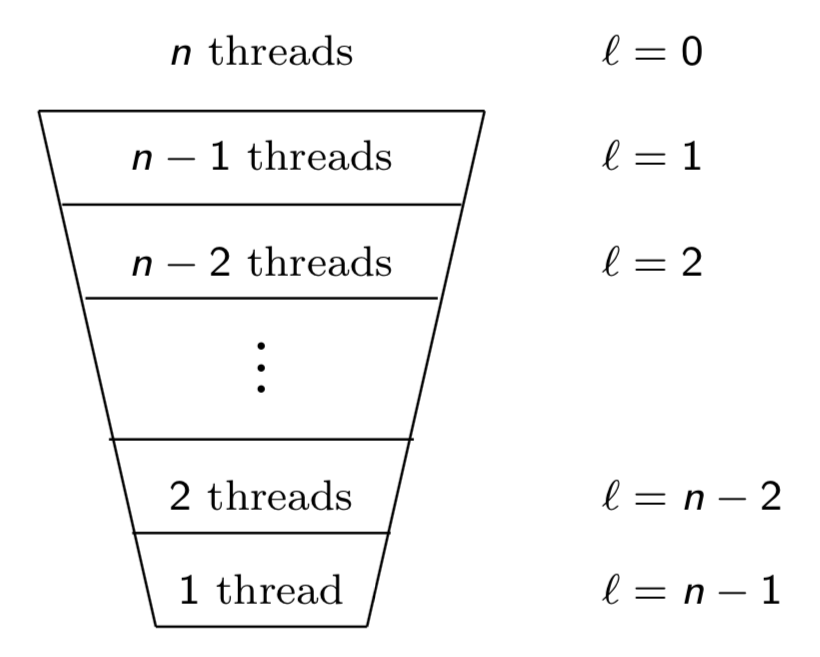
\includegraphics[width=0.5\textwidth]{lecture2/filterlock.png}
\end{center}
For levels $\ell = 1, ..., n-1$ there is a variable \verb|victim[|$\ell$ \verb|]| 
\bigbreak A thread \verb|i| at a level $\ell - 1$ that wants to go to level $\ell$ sets \verb|level[i] =|$\ell$ and \verb|victim[|$\ell$\verb|] = i| 
\bigbreak Thread \verb|i| waits with going to level $\ell$ until either \verb|level[j] <|$\ell$ for all \verb|j|$\neq 1$ or \verb|victim[|$\ell$ \verb|]|$\neq$ \verb|i|.
\bigbreak In other words, thread \verb|i| \textit{spins} on:
\begin{itemize}
    \item \verb|level[j]| for each \verb|j| $\neq$ \verb|i|, to check whether they are all < $\ell$; and
    \item \verb|victim[|$\ell$ \verb|]| to check whether it is $\neq$ \verb|i|
\end{itemize}
The \verb|level[_]| and \verb|victim[_]| fields must be volatile.
\bigbreak Shared counters are useful to have when performing a simple task with multiple threads, as it leads to less memory usage for variables as well as a fairly simple way to synchronize threads. Shared counters have \textbf{risks}: two or more threads could read the value of the counter at the \textit{same time}, and both increment it. Reading a counter and increasing its value are \textit{distinct atomic steps}. Both threads then analyze the value of the counter, while the next value is then skipped.
\\\textbf{Solutions to this}:
\begin{itemize}
    \item \textbf{mutual exclusion} (i.e. a lock), guaranteeing only one thread at a time has access to the counter
    \item use a \textbf{read-modify-write} hardware primitive to turn the process of reading and increasing the counter into a single atomic step
\end{itemize}
\subsection{Mutual Exclusion - Alice and Bob}
Two neighbours A and B share a garden. Alice owns a cat, and Bob owns a dog. The pets must never be in the garden at the same time.
\subsubsection{A simple approach}
\begin{itemize}
    \item look at the garden, see if it is empty.
    \item \textbf{However}, if Alice and Bob look at almost the exact same time, they would both think the garden is empty
    \item We realise that looking at the garden and releasing a pet are two distinct atomic steps
\end{itemize}
\subsubsection{Mobile phone protocol}
\begin{itemize}
    \item One neighbour calls the other prior to releasing their pet
    \item \textbf{However}, the other neighbour may be otherwise away from their phone, or their phone may be out of charge. 
    \item this is an example of \textbf{transient} communication, which is not ideal as recipients can be non-responsive. This would lead to unnecessary waiting with real threads
\end{itemize}
\subsubsection{Can Protocol}
A can on Alice's window-ledge, with a string to Bob's house (and vice versa)
\\Alice pulls the string to knock down Bob's can when she wants to let her pet into the garden (and vice versa).
\\Alice lets her cat into the garden if Bob's can is down and her can is up (and vice versa).
\\This protocol is \textbf{persistent}, instead of transient like before. But Alice relies on Bob to reset his can after her cat has left the yard (and vice versa), which isn't always possible.
\\Interrupts not ideal for solving mutex. Better for A and B to control their own signals.
\subsubsection{Flag Protocol (semaphores)}
A protocol for each individual:
\\\textbf{Alice's protocol}:
\begin{itemize}
    \item raise flag (signalling desire to release pet)
    \item wait until Bob's flag goes down
    \item release pet
    \item after pet has returned, lower flag
\end{itemize}
\textbf{Bob's protocol}:
\begin{itemize}
    \item raise flag
    \item while Alice's flag is up:
    \begin{itemize}
        \item lower flag
        \item wait until Alice's flag is down
        \item raise flag
    \end{itemize}
    \item release pet
    \item after pet has returned, lower flag
\end{itemize}
Bob always yields to Alice, to prevent deadlock. If both Alice and Bob yielded to eachother, we would still experience deadlock.
\\\textbf{Mutual Exclusion}: this method satisifies this condition, as the pets are never in the garden together.
\\\textbf{Deadlock-freeness}: If a pet wants to enter the garden, one of the pets \textit{eventually} succeeds. If only one pet wants to enter the garden, it succeeds. If both want to enter at the same time, Bob sees Alice's raised flag and gives her priority.
\\\textbf{Starvation-freeness}: The flag protocol is not starvation-free. The dog might never get in, while the cat may keep entering and leaving the garden.
\\textbf{Lock-freeness}: The flag protocol is not lock-free. If Bob dies while his flag is raised, the cat may never enter the garden.
\\Mutual exclusion cannot be effectively solved by transient communication, or interrupts. It \textit{can} be solved by MRSW\footnote{Multi-Reader Single-Writer} shared variables.



%
% Lecture 3
%
\section{Concurrent Objects}

\section{Foundations of Shared Memory}

\section{The Relative Power of Primitive Synchronization Operations}

\section{Universality of Consensus}

\section{Spin Locks and Contention}

\section{Monitors and Blocking Synchronization}

\section{Barriers}

\section{Multithreaded Programming}

\section{Linked Lists: The Role of Locking}

\section{Concurrent Queues and Stacks}

\section{Work Distribution, Futures and Scheduling}

\section{Transactional Memory}

\end{document}
